\documentclass[journal,12pt,onecolumn]{IEEEtran}
\usepackage{graphicx, float}
\graphicspath{{Figs/}}
\usepackage{multicol}
\usepackage{parskip}
\usepackage{titlesec}
\usepackage{color}
\usepackage{enumitem}
\usepackage{amsmath,amssymb,amsfonts,amsthm}
\usepackage{array}
\usepackage{booktabs}
\usepackage[table]{xcolor}
\usepackage{longtable}
\usepackage{gensymb}
\usepackage{cite}
\usepackage{algorithmic}
\usepackage{textcomp}
\usepackage{txfonts}
\usepackage{listings}
\usepackage{mathtools}
\usepackage{comment}
\usepackage{tkz-euclide}
\usepackage[breaklinks=true]{hyperref}
\usepackage{gvv}
\usepackage[latin1]{inputenc}
\usetikzlibrary{arrows.meta, positioning}
\usepackage{xparse}
\usepackage{calc}
\usepackage{multirow}
\usepackage{hhline}
\usepackage{ifthen}
\usepackage{lscape}
\usepackage{tabularx}
\usepackage{circuitikz}
\usepackage{tikz}
\newtheorem{problem}{Problem}
\newtheorem{theorem}{Theorem}[section]
\newtheorem{proposition}{Proposition}[section]
\newtheorem{lemma}{Lemma}[section]
\newtheorem{corollary}[theorem]{Corollary}
\newtheorem{example}{Example}[section]
\newtheorem{definition}[problem]{Definition}
\newcommand{\BEQA}{\begin{eqnarray}}
\newcommand{\EEQA}{\end{eqnarray}}
\theoremstyle{remark}
\title{Graduate Aptitude Test in Engineering 2021}
\author{EE25BTECH11025- Vishwambhar}

\begin{document}

\maketitle

\section{\large\textbf{General Aptitude (GA)}}

\begin{enumerate}
\item The current population of a city is 11,02,500. If it has been increasing at the rate of $5\%$ per annum, what was its population 2 years ago?
\begin{enumerate}
    \item 9,92,500
    \item 9,95,006
    \item 10,00,000
    \item 12,51,506
\end{enumerate}
\hfill{(GATE PE 2021)}

\item $p$ and $q$ are positive integers and $\frac{p}{q}+\frac{q}{p}=3$, then, $\frac{p^2}{q^2}+\frac{q^2}{p^2}=$
\begin{enumerate}
\begin{multicols}{4}
    \item 3
    \item 7
    \item 9
    \item 11
\end{multicols}
\end{enumerate}
\hfill{(GATE PE 2021)}

\item The least number of squares that must be added so that the line P-Q becomes the line of symmetry is \dots
\begin{figure}[h]
    \centering
    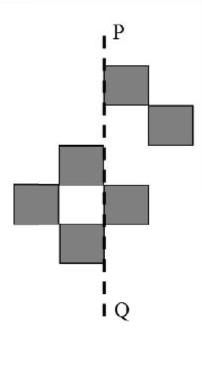
\includegraphics[width=0.2\columnwidth]{Q_3.png}
    \caption{}
    \label{fig:placeholder}
\end{figure}
\begin{enumerate}
\begin{multicols}{4}
    \item 4
    \item 3
    \item 6
    \item 7
\end{multicols} 
\end{enumerate}
\hfill{(GATE PE 2021)}

\item $Nostalgia$ is to $anticipation$ as \dots is to \dots\\
Which one of the following options maintains a similar logical relation in the above sentence?
\begin{enumerate}
    \item Present, past
    \item Future, past
    \item Past, future
    \item Future, present
\end{enumerate}
\hfill{(GATE PE 2021)}

\item Consider the following sentences:\\
(i)I woke up from sleep\\
(ii)I woked up from sleep\\
(iii)I was woken up from sleep\\
(iv)I was wokened up from sleep\\
Which one of the above sentences are grammatically \textbf{CORRECT}?
\begin{enumerate}
    \item (i) and (ii)
    \item (i) and (iii)
    \item (ii) and (iii)
    \item (i) and (iv)
\end{enumerate}
\hfill{(GATE PE 2021)}

\item Given below are two statements and two conclusions.\\
Statement I: All purple are green.\\
Statement II: All black are green.\\
Conclusion I: Some black are purple.\\
Conclusion II: No black are purple.\\
Based on the above statements and conclusions, which one of the following options is logically \textbf{CORRECT}?
\begin{enumerate}
    \item Only conclusion I is correct.
    \item Only conclusion II is correct.
    \item Either conclusion I or II is correct.
    \item Both conclusion I and II are correct.
\end{enumerate}
\hfill{(GATE PE 2021)}

\item Computers are ubiquitous. They are used to improve efficiency in almost all fields from agriculture to space exploration. Artificial intelligence(AI) is currently a hot topic. AI enables computers to learn, given enough training date. For humans, sitting in front of a computer for long hours can lead to health issues.\\
Which one of the following can be deduced from the above passage?\\
(i)Nowadays, computers are present in almost al places.\\
(ii)Computers cannot be used for solving problems in engineering.\\
(iii)For humans, there are both positive and negative effects of using computers.\\
(iv)Artificial intelligence can be done without data.
\begin{enumerate}
    \item (ii) and (iii)
    \item (ii) and (iv)
    \item (i), (iii) and (iv)
    \item (i) and (iii)
\end{enumerate}
\hfill{(GATE PE 2021)}

\item Consider a square sheet of side 1 unit. In the first step, it is cut along the main diagonal to get two triangles. In the next step, one of the cut triangles is revolved about its short edge to form a solid cone. The volume of the resulting cone, in cubic units, is \dots
\begin{enumerate}
\begin{multicols}{4}
     \item $\frac{\pi}{3}$
     \item $\frac{2\pi}{3}$
     \item $\frac{3\pi}{2}$
     \item $3\pi$
\end{multicols}
\end{enumerate}
\hfill{(GATE PE 2021)}

\item The number of minutes spent by two students, \textbf{X} and \textbf{Y}, exercising every day in given week are shown in the bar chart above.\\
The number of days in the given week in which one of the students spent a minimum of 10$\%$ more than the other student, on a given day, is
\begin{figure}[h]
    \centering
    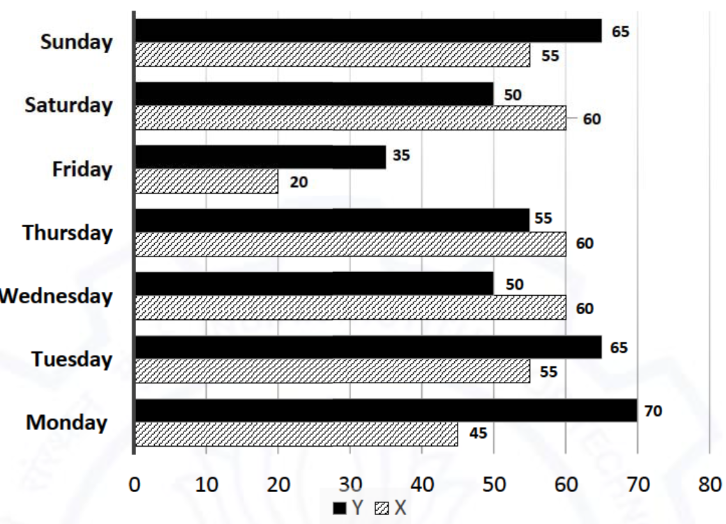
\includegraphics[width=0.5\columnwidth]{Q_9.png}
    \caption{}
    \label{fig:placeholder}
\end{figure}
\begin{enumerate}
\begin{multicols}{4}
    \item 4
    \item 5
    \item 6
    \item 7
\end{multicols}
\end{enumerate}
\hfill{(GATE PE 2021)}

\item Corners are cut from an equilateral triangle to produce a regular convex hexagon as shown in the figure above.\\
The ratio of the area of the regular convex hexagon to tha area of the original equilateral triangle is 
\begin{figure}[h]
    \centering
    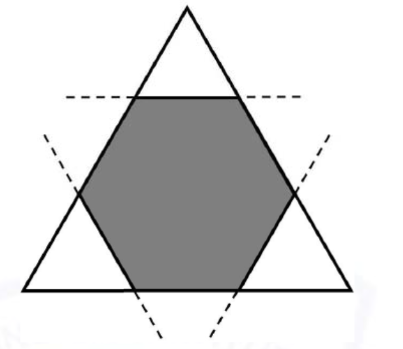
\includegraphics[width=0.2\columnwidth]{Q_10.png}
    \caption{}
    \label{fig:placeholder}
\end{figure}
\begin{enumerate}
\begin{multicols}{4}
    \item $2:3$
    \item $3:4$
    \item $4:5$
    \item $5:6$
\end{multicols}
\end{enumerate}
\hfill{(GATE PE 2021)}

\end{enumerate}

\section{\large\textbf{Petroleum Engineering(PE)}}

\begin{enumerate}
\item MOPU (in the context of offshore drilling and production systems) stands for
\begin{enumerate}
    \item Mobile Offshore Process Unit
    \item Mobile Offshore Piping Unit
    \item Mobile Offshore Production Unit
    \item Mobile Oil Production Unit
\end{enumerate}
\hfill{(GATE PE 2021)}

\item Which ONE of the following statements is \textbf{INCORRECT}?
\begin{enumerate}
    \item Conductor is the outer casing of a well
    \item Riser is used for transporting fluid
    \item Conductor and riser have the same functions
    \item Conductor is used for shielding the well flow lines from external forces
\end{enumerate}
\hfill{(GATE PE 2021)}

\item Which ONE of the following offshore installations uses Dynamic Positioning System (DPS) for the station keeping?
\begin{enumerate}
    \item Jacket 
    \item Jacket-up
    \item Semi- submersible
    \item Tension Leg Platform
\end{enumerate}
\hfill{(GATE PE 2021)}

\item  Which one of the following is \textbf{NOT} a primary safety system for offshore installation?
\begin{enumerate}
    \item Emergency Shut Down
    \item Isolation
    \item Fire Protection
    \item Blowdown
\end{enumerate}
\hfill{(GATE PE 2021)}

\item The primary function of the thruster in the Dynamic Positioning System (DPS) of an offshore installation is
\begin{enumerate}
    \item To apply thrust in the direction opposite to the resultant environmental force
    \item To apply thrust in the same direction as the resultant environmental force
    \item To apply thrust in the direction opposite to the motion
    \item To apply thrust in the same direction as the motion
\end{enumerate}
\hfill{(GATE PE 2021)}

\item Select the \textbf{CORRECT} firefighting system for electrical switchgear room an offshore facility.
\begin{enumerate}
    \item Wet chemical
    \item Halon system
    \item Foam
    \item Water sprinklers
\end{enumerate}
\hfill{(GATE PE 2021)}

\item Which one of the following options can be used to quantify secondary porosity?
\begin{enumerate}
    \item Sonic and Gamma Ray Logs
    \item Sonic and Neutron Logs
    \item Sonic and Caliper Logs
    \item Density and Neutron Logs
\end{enumerate}
\hfill{(GATE PE 2021)}

\item Among the options given below, what is the typical temperature range for significant oil generation in a source rock associated with conventional crude-oil reservoirs?
\begin{enumerate}
    \item $10\degree C-40\degree C$
    \item $60\degree C-175\degree C$
    \item $225\degree C-325\degree C$
    \item $350\degree C-425\degree C$
\end{enumerate}
\hfill{(GATE PE 2021)}

\item In the original Darcy's law as proposed by Henry Darcy, which of the following drives the fluid flow through a fully saturated sand column?
\begin{enumerate}
    \item Pressure-gradient or hydraulic-gradient
    \item Viscous force per unit volume
    \item Capillary force per unit volume
    \item Inertial force per unit volume
\end{enumerate}
\hfill{(GATE PE 2021)}

\item At which one of the following scales is Darcy's law for fluid flow through a porous medium applicable?
\begin{enumerate}
    \item Nano-scale
    \item Molecular-scale
    \item Microscopic-scale
    \item Macroscopic-scale
\end{enumerate}
\hfill{(GATE PE 2021)}

\item Pressure-Temperature phase diagram of $CO_2$ is shown below. Identify the correct phases from the given options.
\begin{figure}[h]
    \centering
    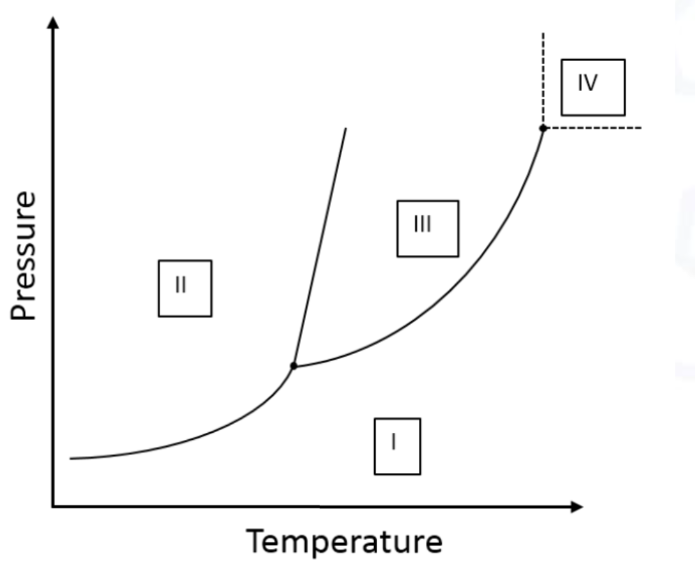
\includegraphics[width=0.5\columnwidth]{Q_11.png}
    \caption{}
    \label{fig:placeholder}
\end{figure}
\begin{enumerate}
    \item I = Solid Phase, II = Liquid Phase, III = Gas Phase, IV = Supercritical Phase
    \item I = Gas Phase, II = Supercritical Phase, III = Solid Phase, IV = Liquid Phase
    \item I = Supercritical Phase, II = Liquid Phase, III = Solid Phase, IV = Gas Phase
    \item I = Gas Phase, II = Solid Phase, III = Liquid Phase, IV = Supercritical Phase
\end{enumerate}
\hfill{(GATE PE 2021)}

\item A measure of the potential of crude oil to form surfactants for Enhanced Oil Recovery (EOR) is given by the Total Acid Number (TAN). TAN is the mass of \dots (in milligrams) that is required to neutralize one gram of crude oil.
\begin{enumerate}
    \item $Ca(OH)_2$
    \item $NaCl$
    \item $KOH$
    \item $NaOH$
\end{enumerate}
\hfill{(GATE PE 2021)}

\item In Water-Alternating-Gas (WAG) injection, the purpose of the injection is to \dots I \dots the "relative permeability" of gas and to \dots II \dots the "mobility" of the gas.
\begin{enumerate}
    \item I = reduce, II = enhance
    \item I = reduce, II = reduce
    \item I = enhance, II = reduce
    \item I = enhance, II = enhance
\end{enumerate}
\hfill{(GATE PE 2021)}

\item Solids that may possibly form in the offshore pipelines during the production of oil and gas from deep-water reservoirs are
\begin{enumerate}
    \item Wax
    \item Char
    \item Hydrates
    \item Asphaltenes
\end{enumerate}
\hfill{(GATE PE 2021)}

\item Oil and gas pipelines, which are at an elevated pressure (about 3 MPa) and sub-ambient temperature (below 298 K), may get blocked by the formation of solid hydrates. One of the strategies adopted to inhibit the formation of hydrates is the injection of Thermodynamic Hydrate Inhibitors (THIs) into the reservoir fluid.\\
Identify all suitable chemicals that are commonly used as THIs.
\begin{enumerate}
    \item Sodium Chloride
    \item Methanol
    \item Polyvinylpyrrolidone
    \item Sodium Dodecyl Sulphate
\end{enumerate}
\hfill{(GATE PE 2021)}

\item When $CO_2$ and liquid water are brought in contact with each other, they may form solid hydrates. The three-phase hydrate boundary is shown in the Pressure-Temperature plot given below.\\

Identify the correct statements.\\

G = Gas Phase, H = Hydrate Phase, L = Liquid Phase
\begin{figure}[h]
    \centering
    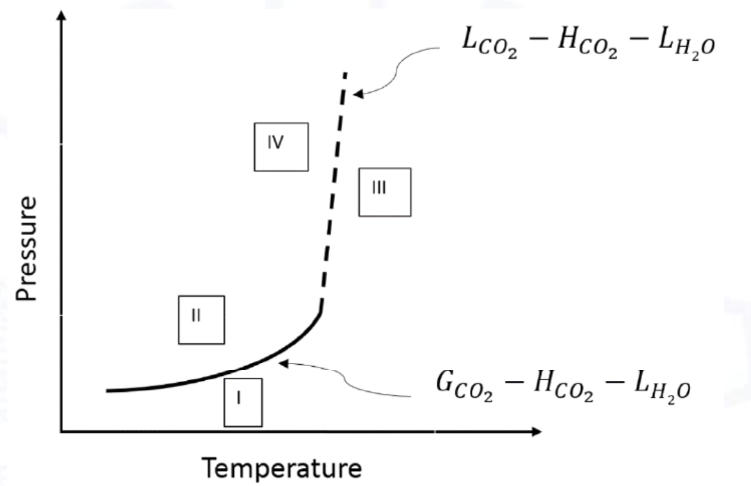
\includegraphics[width=0.5\columnwidth]{Q_16.png}
    \caption{}
    \label{fig:placeholder}
\end{figure}
\begin{enumerate}
    \item Hydrates are stable in region I
    \item Hydrates are stable in region II
    \item Hydrates are stable in region III
    \item Hydrates are stable in region IV
\end{enumerate}
\hfill{(GATE PE 2021)}

\item Heavy oil recovered from reservoirs can be represented by $C_XH_{1.5X}$ Suitable processes to reduce the density of heavy oil are
\begin{enumerate}
    \item Carbon Rejection
    \item Pyrolysis
    \item Hydrogenation
    \item Filtration
\end{enumerate}
\hfill{(GATE PE 2021)}

\item Identify the \textbf{CORRECT} statements for a $n\times n$ matrix.
\begin{enumerate}
    \item Under elementary row operations, the rank of the matrix remains invariant
    \item Under elementary row operations, the eigenvalues of the matrix remain the same
    \item  If the elements in a row can be written as a linear combination of two or more rows, then the matrix is singular.
    \item The rank of the matrix is equal to n if the determinant of the matrix is zero.
\end{enumerate}
\hfill{(GATE PE 2021)}

\item During a drilling operation, kick occurs if
\begin{enumerate}
    \item the shear ram in the Blow Out Preventer (BOP) does not work.
    \item the formation pressure is equal to the drilling fluid pressure.
    \item the volume of the mud used to fill the hole is less than that of the pipe being pulled out.
    \item the formation pressure is more than the drilling fluid pressure.
\end{enumerate}
\hfill{(GATE PE 2021)}

\item The value of $\lim\limits_{x \to 0} \frac{4x^3-2x^2+x}{3x^2+2x}$ is \dots(correct up to one decimal place).\\

\hfill{(GATE PE 2021)}

\item Given two complex numbers, $Z_1=4+3i$ and $Z_2=2-5i$, the real part of ($Z_1Z_2$) is \dots\\

\hfill{(GATE PE 2021)}

\item The number of 'three-digit numbers' that can be formed using the digits from 1 to 9 without the repetition of each digit is \dots\\

\hfill{(GATE PE 2021)}

\item The estimate for the root of the function $f\brak{x}=e^{2x}+2x$ after one iteration with an initial guess of $x_0=0$, using the Newton-Raphson method is \dots(correct up to two decimal places).\\

\hfill{(GATE PE 2021)}

\item A saturated oil reservoir has an average reservoir pressure of 3000 psia, tested for flowing bottom-hole pressure (BHP) of 2000 psia and production rate of 500 STB/day. The maximum reservoir deliverability based on Vogel's equation for two-phase flow is \dots  STB/day.\\

\hfill{(GATE PE 2021)}

\item If the specific heat ratio of natural gas is 1.28, the critical pressure ratio (ratio of outlet pressure to upstream pressure) through a choke is \dots (round off to two decimal places).\\

\hfill{(GATE PE 2021)}

\item Match the suitable artificial lift methods to meet the requirements given in the table.\\
\begin{tabular}{ll}
(P) Progressive cavity pump & (I) To deliver high-water cut (95\%) oil with high flow rate. \\
(Q) Electric submersible pump & (II) Increase the viscosity of the aqueous phase \\
(R) Sucker rod pump & (III) To deliquify a gas-well with 5 bbl/day water. \\
(S) Gas lift & (IV) To be used in a sandy oil well to produce 5000 bbl/day. \\
\end{tabular}
\begin{enumerate}
    \item P - I, Q - II, R - IV, S - III \\
    \item P - II, Q - I, R - IV, S - III \\
    \item P - I, Q - II, R - III, S - IV \\
    \item P - II, Q - I, R - III, S - IV
\end{enumerate}
\hfill{(GATE PE 2021)}

\item Match the Enhanced Oil Recovery (EOR) methods with the corresponding laboratory tests.\\
\begin{tabular}{ll}
(P) Gas injection EOR & (I) Interfacial tension studies \\
(Q)  In-situ combustion EOR & (II) Screen viscometer test \\
(R) Polymer flooding EOR & (III) Minimum miscibility pressure test \\
(S) Surfactant-Alkaline EOR & (IV) Oxidation cell test \\
\end{tabular}
\begin{enumerate}
    \item P - III, Q - II, R - I, S - IV \\
    \item P - II, Q - IV, R - I, S - III \\
    \item P - III, Q - IV, R - II, S - I \\
    \item P - II, Q - IV, R - II, S - I
\end{enumerate}
\hfill{(GATE PE 2021)}

\item Identify the following well test methods corresponding to the transient pressure profiles in the figures given below. (BHP: Bottom-hole pressure, BOPD: Barrels of oil per day)\\

(P) Flow-after-flow test\\
(Q) Interference test\\
(R) Fall-off test\\
(S) Modified isochronal test\\
\begin{figure}[h]
    \centering
    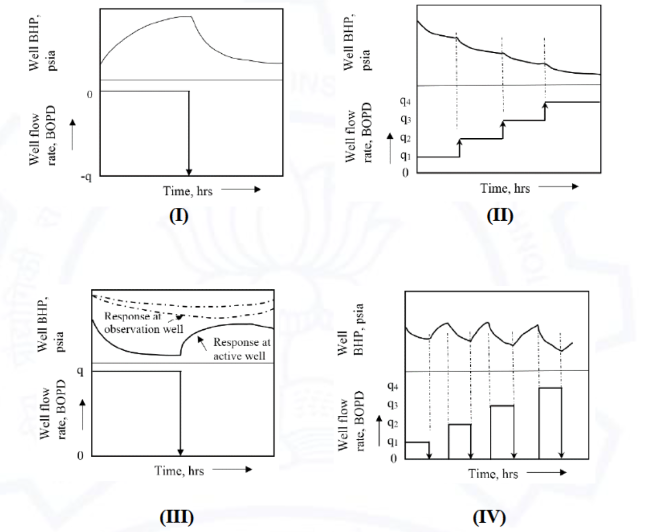
\includegraphics[width=0.5\columnwidth]{Q_28.png}
    \caption{}
    \label{fig:placeholder}
\end{figure}
\begin{enumerate}
    \item P - IV, Q - II, R - I, S - III
    \item P - II, Q - III, R - IV, S - I
    \item P - III, Q - III, R - I, S - IV
    \item P - IV, Q - I, R - III, S - II
\end{enumerate}
\hfill{(GATE PE 2021)}

\item Match the following wire-line logging methods based on the physical principles of measurements.\\
\begin{tabular}{ll}
(P) Induction Log & (I) Measures natural radioactivity of a formation\\
(Q) Gamma-Ray Log & (II) Measures induced magnetic moment of hydrogen nuclei (protons)\\
(R) Sonic Log & (III) Measures electrical resistivity/conductivity. \\
(S) Nuclear Magnetic Resonance Log & (IV) Measures elastic wave propagation properties. \\
\end{tabular}
\begin{enumerate}
    \item P - II, Q - I, R - IV, S - III \\
    \item P - III, Q - I, R - IV, S - II \\
    \item P - III, Q - II, R - IV, S - I \\
    \item P - III, Q - I, R - III, S - IV
\end{enumerate}
\hfill{(GATE PE 2021)}

\item Match the following rock types with their respective chemical compositions from the given options.\\
\begin{tabular}{ll}
(P) Sandstone & (I) A non-clastic carbonate rock consisting mainly of the mineral calcite.\\
(Q) Limestone & (II) A non-clastic chemical rock composed of mineral halite.\\
(R) Shale & (III) A siliciclastic rock formed mainly of sand. \\
(S) Rock salt & (IV) A fissile rock with a laminated structure, formed by consolidation of clay or mud. \\
\end{tabular}
\begin{enumerate}
    \item P - III, Q - II, R - IV, S - I \\
    \item P - II, Q - III, R - I, S - IV \\
    \item P - III, Q - I, R - IV, S - II\\
    \item P - III, Q - I, R - II, S - IV
\end{enumerate}
\hfill{(GATE PE 2021)}

\item The following equations describe the transient fluid flow in a typical petroleum reservoir system. Here, p is pressure, x and r are the spatial coordinates in rectangular and cylindrical systems respectively, and t is time. Also, $\phi$ (porosity), $\mu$ (viscosity), $c_f$ (formation compressibility), $c_t$ (total compressibility) and $k$ (permeability) are constant coefficients.\\
Match the equations with their corresponding descriptions.\\
\begin{tabular}{ll}
(P) $\frac{\partial^2 p}{\partial r^2}+\frac{1}{r}\frac{\partial p}{\partial r}=\frac{\phi\mu c_t}{k}\frac{\partial p}{\partial t}$ & (I) Equation in Cartesian coordinates used to describe incompressible fluid flow\\
(Q) $\frac{\partial^2p}{\partial x^2}=\frac{\phi \mu c_t}{k}\frac{\partial p}{\partial t}$ & (II)  Equation in Cartesian coordinates used to describe slightly compressible fluid flow.\\
(R) $\frac{\partial^2p}{\partial x^2}+c_f\brak{\frac{\partial p}{\partial    x}}^2=\frac{\phi \mu c_t}{k}\frac{\partial p}{\partial t}$& (III) Equation in cylindrical coordinates used to describe slightly compressible fluid flow \\
(S) $\frac{\partial^2p}{\partial r^2}+\frac{1}{r}\brak{\frac{\partial p}{\partial r}}+c_f\brak{\frac{\partial p}{\partial r}}^2=\frac{\phi \mu c_t}{k}\frac{\partial p}{\partial t}$& (IV) Equation in cylindrical coordinates used to describe incompressible fluid flow \\
\end{tabular}
\begin{enumerate}
    \item P - IV, Q - I, R - II, S - III \\
    \item P - IV, Q - III, R - II, S - I \\
    \item P - III, Q - IV, R - II, S - I\\
    \item P - III, Q - IV, R - I, S - II
\end{enumerate}
\hfill{(GATE PE 2021)}

\item Select the \textbf{INCORRECT} statement related to Enhanced Oil Recovery (EOR) techniques from the following options
\begin{enumerate}
    \item Alkaline flooding recovers crude oil by reduction of interfacial tension (IFT) and reversal of wettability of rocks.
    \item In-situ combustion recovers crude oil by the application of heat, thus lowering the viscosity of the crude oil.
    \item Nitrogen flue gas flooding recovers crude oil by vaporizing the lighter components of the crude oil.
    \item Polymer flooding recovers crude oil by reducing the viscosity and increasing the mobility of water
\end{enumerate}
\hfill{(GATE PE 2021)}

\item Match the petroleum reservoir forming traps with their general classifications.\\
\begin{tabular}{ll}
(P)  Dome and Anticlinal Trap& (I) A geological structure with bodies of porous lithofacies embedded in impermeable lithofacies.\\
(Q) Salt Dome& (II) A geological structure formed by the tectonic uplift and/or folding of sedimentary rocks\\
(R)  Fault Trap & (III) A geological structure caused by the upward intrusion of a diapiric body of halite. \\
(S) Lenticular Trap & (IV) A geological plane with a sealing effect that acts as a fluid migration barrier for reservoir rocks \\
\end{tabular}
\begin{enumerate}
    \item P - III, Q - II, R - IV, S - I \\
    \item P - II, Q - III, R - IV, S - I\\
    \item P - III, Q - I, R - II, S - IV\\
    \item P - II, Q - III, R - I, S - IV
\end{enumerate}
\hfill{(GATE PE 2021)}

\item An Ideal Pressure Buildup Test yields a single straight line for all times, when shut-in Bottom-Hole Pressure $\brak{P_{ws}}$ is plotted against
$\log_{10}\frac{\brak{t_p+\triangle t }}{\triangle t}$. Here $t_p$ is the well production time and $\triangle t$ is the time elapsed since shut-in. However, in an actual Pressure Buildup Test, a non-linear curve is obtained which can be logically divided into distinct regions.
Choose \textbf{INCORRECT} option from the following.
\begin{enumerate}
    \item A late-time region, in which the radius of investigation has reached the well's drainage boundaries
    \item A middle-time region during which the pressure transient has moved away from the wellbore and into the bulk formation
    \item An early-time region during which a pressure transient is moving through the formation nearest the wellbore.
    \item An early-time region during which a pressure transient is moving away from the drainage boundary
\end{enumerate}
\hfill{(GATE PE 2021)}

\item When two immiscible fluid phases are placed in contact with a solid surface, one phase usually is attracted to solid more strongly than the other phase. The more strongly attracted phase is called the 'wetting phase'.\\
The inter-molecular interaction of the non-wetting phase with the solid is \dots I\dots  than its intra-molecular interaction. Due to this, the non-wetting phase tends to occupy the \dots II\dots of the reservoir.
\begin{enumerate}
    \item I = stronger, II = smaller pores
    \item I = stronger, II = larger pores
    \item I = weaker, II = smaller pores.
    \item I = weaker, II = larger pores
\end{enumerate}
\hfill{(GATE PE 2021)}

\item Coal bed methane is methane gas adsorbed in coal seams. To desorb the methane from the coal seam it should be exposed to $CO_2$ and (or) $N_2$. Which ONE of the following is an appropriate reason to enhance the desorption process?\\
\begin{enumerate}
    \item $N_2$ is used because it has low kinetic energy compared to $CH_4$
    \item $CO_2$ is used as it has high kinetic energy compared to $CH_4$
    \item $CO_2$ is used as it strongly binds with coal compared to $CH_4$
    \item $N_2$. is used as it strongly binds with coal compared to $CH_4$
\end{enumerate}
\hfill{(GATE PE 2021)}

\item Match the platforms with appropriate support systems\\
\begin{tabular}{ll}
(P) Semi-submersible& (I) Tether.\\
(Q) Spar platform& (II) Turret Mooring\\
(R) Tension leg platform& (III) Catenary Mooring \\
(S) FPSO & (IV) Column Stabilised Unit \\
\end{tabular}
\begin{enumerate}
    \item P - IV, Q - III, R - I, S - II \\
    \item P - II, Q - III, R - I, S - IV\\
    \item P - III, Q - I, R - IV, S - II\\
    \item P - I, Q - IV, R - II, S - III
\end{enumerate}
\hfill{(GATE PE 2021)}

\item Select the \textbf{CORRECT} statements from the following.\\
Well testing operations on a typical crude oil reservoir\\
\begin{enumerate}
    \item do not measure rock and fluid properties of the reservoir when the well is flowing or shut-in.
    \item measure variation in pressure response of the reservoir with time when the well is flowing or shut-in.
    \item measure productivity index and partial well completion.
    \item do not measure length and conductivity of hydraulic fractures.
\end{enumerate}
\hfill{(GATE PE 2021)}

\item Crude oil from oil sands contains bitumen and asphaltene and this crude is heavy and viscous at room temperature. Assume that one such crude oil is represented by $C_X H_{1.2X}O_Y$. For easier transportation through pipelines it should be processed further. Identify the processes which help in transportation of this crude oil.
\begin{enumerate}
    \item Drying
    \item Vis-breaking
    \item Coking process
    \item Hydro-treating
\end{enumerate}
\hfill{(GATE PE 2021)}

\item Given matrix $A=\myvec{
2&-1\\
-1&2}$. The eigenvalue corresponding to the eigenvector $\myvec{1\\
-1}$ is \dots \\

\hfill{(GATE PE 2021)}

\item The maximum value of the function $f\brak{x}=x^4-8x^2+2$ for $-2\leq x \leq 2$ is \dots\\

\hfill{(GATE PE 2021)}

\item Given the second order ordinary differential equation: $y''+3y'-4y=0$ with the initial condition $y\brak{0}=3$, and $y'\brak{0}=-7$, the value  of $y\brak{1}$ is \dots(round off to two decimal places)\\

\hfill{(GATE PE 2021)}

\item The directional derivative of $f\brak{x,y,z}=x^2+3y^2+z^2$, at point $\brak{2,1,0}$ along the unit vector in $x$-direction, $\vec{i}$, is \dots \\

\hfill{(GATE PE 2021)}

\item A productivity test conducted on a crude oil well indicates a stabilized flow rate of 150 STB/day (water-free oil production) at a bottom-hole flowing pressure of 935 psig. After shutting the well for 24 hours, the bottom-hole pressure reached a static value of 1250 psig.\\
The Absolute Open Flow (AOF) potential of the well is \dots STB/day.\\

\hfill{(GATE PE 2021)}

\item A porous medium (shown schematically in the figure) has the following properties.\\
Length$=600m$, Width $=8m$, Height $=0.5m$, Permeability $k=100mD$, Porosity $\phi=15\%$.
\begin{figure}[h]
    \centering
    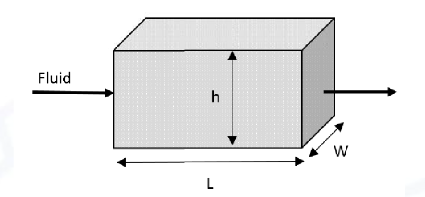
\includegraphics[width=0.5\linewidth]{Q_45.png}
    \caption{}
    \label{fig:placeholder}
\end{figure}
An incompressible fluid having a viscosity of 2 cP is flowing through a porous medium at the inlet and exit pressures of $7\times 10^6$ Pa and $6\times 10^6$ Pa, respectively.
The actual fluid velocity through the porous medium is \dots $\times 10^{-7}$ m/s.
(1 Darcy = $10^{-12} m^2$)\\

\hfill{(GATE PE 2021)}

\item A tubing with an inner diameter of 2.259 inch delivers oil from a well at the rate of 1000 bbl/day. The API gravity and viscosity of the oil are $40\degree$ and 1.2 cP, respectively. The tubing makes an angle of $15\degree$ with the vertical. Assuming a fanning friction factor of $0.006$, the pressure-drop over a length of 1000 ft tubing is \dots psi (round off to nearest integer).\\
$[1bbl =5.615 ft^2]$ \\

\hfill{(GATE PE 2021)}

\item A cylindrical crude oil reservoir with a radius of 3000 ft is under water influx from a cylindrical aquifer with an estimated radius of 9000 ft. The reservoir has the following properties.\\
Aquifer thickness $h=40ft$\\
Porosity, $\phi=15\%$\\
Formation compressibility, $C_f=4.5\times 10^{-6}psi^{-1}$\\
Water compressibility, $C_w=4.0\times10^{-6}psi^{-1}$\\
Assuming a pot reservoir model with fractional encroachment angle as unity, the water influx into the reservoir for a pressure drop of 700 psi is \dots MMbbl (million barrels) (round off to two decimal places).
($\pi=3.14$, 1 bbl $=5.615ft^3$)\\

\hfill{(GATE PE 2021)}

\item A heavy oil reservoir with an initial oil recovery of 10\% has the following properties.\\
Confined area A = 1.5 acres, thickness of the reservoir h = 15 ft,\\
effective porosity $\phi$ = 15\%, irreducible water saturation $S_{wr}$ = 25\%,\\
oil formation volume factor $B_0$ = 1.10 bbl/STB.\\
An in-situ combustion test was conducted in the above reservoir. Oil recovery due to the combustion process at the well is observed to be 12000 bbl.\\
The total (overall) oil recovery at the end of the in-situ combustion process is \dots\% (round off to nearest integer) of the original oil in place.\\

(1 acre $=43560ft^2$, 1 bbl $=5.615ft^3$)\\

\hfill{(GATE PE 2021)}

\item A double acting duplex pump with a rod diameter of 2.5 inch and a stroke of 20 inch is to be operated at 60 strokes per minute for drilling down to 10000 ft. The flow rate is 600 gpm. If the volumetric efficiency of the pump is 80\%, the liner size is \dots inch (round off to one decimal place).\\
(1 gallon $=231inch^3$)\\

\hfill{(GATE PE 2021)}

\item The fluid flow through an under-saturated oil reservoir is driven by solution gas drive mechanism. The reservoir parameters are as given below.\\
Compressibility of water, $C_w=1\times10^{-6}psi^{-1}$\\
Compressibility of formation, $C_f=1\times10^{-5}$\\
Connate water saturation, $S_{wc}=0.2$\\
Initial reservoir pressure, $p_i=4000psi$\\
Reservoir pressure at bubble-point, $P_b=3000psi$\\
Oil formation volume factor, $B_{oi}=1.24rb/$\\ 
Formation volume factor at bubble point pressure, $b_{ob}=1.26rb/STB$\\
The percentage of oil recovered as a fraction of the Original Oil in Place (OOIP) is \dots \% (round off to one decimal place).\\

\hfill{(GATE PE 2021)}

\item During drilling, a well is damaged out to a radial distance of 5 ft from the periphery of the wellbore so that the permeability within the damaged zone is reduced to $1/50^{th}$ of the undamaged effective permeability. After completion, the well is stimulated so that the permeability out to a radial distance of 15 ft from the periphery of the wellbore is increased to twenty times the permeability of the undamaged zone.\\
The radial inflow equation for stabilized flow conditions under semi-steady state conditions is given by\\
$p_e-p_{wf}=\frac{q\mu}{2\pi k_eh}\sbrak{ln\brak{\frac{r_e}{r_w}}-\frac{1}{2}+S}$,\\
where $p_e$ is effective pressure, $p_{wf}$ is flowing bottom-hole pressure, $q$ is flow-rate, $\mu$ is viscosity, $k_e$ is average effective permeability, $h$ is reservoir thickness, $r_e$ is drainage radius, $r_w$ is wellbore radius and $S$ is skin factor.\\
If $r_w=0.5ft$ and $r_e=500ft$, then the increase in Productivity Index ratio $\brak{=\frac{PI_{stimulated-well}}{PI_{unstimulated-well}}}$ is \dots
(round off to one decimal place).\\

\hfill{(GATE PE 2021)}

\item A depleted and shut-in oil reservoir originally contained $25\times10^6$ STB of oil with a formation volume factor of 1.35 res bbl/STB and a connate water saturation of 0.25. Cumulative oil production to date has been $2.5\times10^6$ STB of oil. The oil formation volume factor is now 1.25 res bbl/STB. Assuming no water influx, the gas saturation in the reservoir is \dots \% (round off to one decimal place).\\

\hfill{(GATE PE 2021)}

\item Surface tension of liquid A in a capillary is being measured in the laboratory using capillary rise (refer the figure given below). The capillary radius $\brak{r}$ is 100 $\mu m$, the height of liquid column $\brak{h}$ is 10 cm and $\theta=38\degree$. Density of air can be neglected. Assume liquid A to have the same density as water.\\
Surface tension of liquid A at room temperature is \dots dynes/cm (round off to one decimal place).\\
\begin{figure}[h]
    \centering
    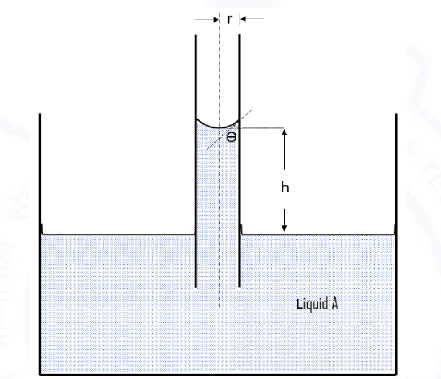
\includegraphics[width=0.5\columnwidth]{Q_53.png}
    \caption{}
    \label{fig:placeholder}
\end{figure}

\hfill{(GATE PE 2021)}

\item Miscible displacement process is one of the EOR techniques. The performance of this process depends on fluid physical properties that affect flow behavior in a reservoir. Two of the important properties are density and viscosity. Consider the use of $CO_2$ for one such process. The density of $CO_2$ at the reservoir condition is \dots $lb/ft^3$ (round off to one decimal place).\\
Relevant data for this calculation are given below.\\
Reservoir temperature = $300\degree F\brak{422K}$\\
Reservoir temperature = $1470 psig \brak{100atm}$\\
Compressibility factor $\brak{z}$ at the reservoir condition $=0.5$\\
Values of universal gas constant $\brak{R}$ in different units are listed below.\\
Universal Gas Constant $\brak{R}=8.314m^3.Pa.K^{-1}.mol^{-1}=10.731psi.ft^3.lb.mol^{-1}\degree R^{-1}=0.082L.atm.K^{-1}mol^{-1}$\\

\hfill{(GATE PE 2021)}

\item In a counter current heat exchanger, the hot fluid enters at $175\degree F$ and exits at $100\degree F$. The cold fluid enters at $175\degree F$ and exits at $75\degree F$. For the calculation of heat transfer rate, consider the tube surface area (per unit length) to be $0.26ft^2/ft$ and a tube length of $ft$. The overall heat transfer coefficient of the exchanger is $100 BTU/hr-ft^2$. The minimum number of tubes required in the exchanger for a heat duty of $15\times10^5BTU/hr$ is \dots (round off to nearest integer).\\

\hfill{(GATE PE 2021)}

\newpage

\begin{tabular}[12pt]{|c|c|c|c|c|c|c|}
\hline
Q. No.&Session&Question Type&Section&Answer&Marks&Negative Marks\\
\hline
1&4&MCQ&GA&C&1&1/3\\
\hline
2&4&MCQ&GA&B&1&1/3\\
\hline
3&4&MCQ&GA&C&1&1/3\\
\hline
4&4&MCQ&GA&C&1&1/3\\
\hline
5&4&MCQ&GA&B&1&1/3\\
\hline
6&4&MCQ&GA&C&1&1/3\\
\hline
7&4&MCQ&GA&D&1&1/3\\
\hline
8&4&MCQ&GA&A&1&1/3\\
\hline
9&4&MCQ&GA&C&1&1/3\\
\hline
10&4&MCQ&GA&A&1&1/3\\
\hline
1&4&MCQ&PE&C&1&1/3\\
\hline
2&4&MCQ&PE&C&1&1/3\\
\hline
3&4&MCQ&PE&C&1&1/3\\
\hline
4&4&MCQ&PE&C&1&1/3\\
\hline
5&4&MCQ&PE&A/C&1&1/3\\
\hline
6&4&MCQ&PE&B&1&1/3\\
\hline
7&4&MCQ&PE&B&1&1/3\\
\hline
8&4&MCQ&PE&B&1&1/3\\
\hline
9&4&MCQ&PE&A&1&1/3\\
\hline
10&4&MCQ&PE&D&1&1/3\\
\hline
11&4&MCQ&PE&D&1&1/3\\
\hline
12&4&MCQ&PE&C&1&1/3\\
\hline
13&4&MCQ&PE&B&1&1/3\\
\hline
14&4&MSQ&PE&A,C,D&1&1/3\\
\hline
15&4&MSQ&PE&A,B&1&1/3\\
\hline
16&4&MSQ&PE&B,D&1&1/3\\
\hline
17&4&MSQ&PE&A,C/A,B,C&1&1/3\\
\hline
18&4&MSQ&PE&A,C&1&1/3\\
\hline
19&4&MSQ&PE&C,D/D&1&1/3\\
\hline
20&4&NAT&PE&0.5&1&1/3\\
\hline
21&4&NAT&PE&-7&1&1/3\\
\hline
22&4&NAT&PE&504&1&1/3\\
\hline
23&4&NAT&PE&-0.25&1&1/3\\
\hline
24&4&NAT&PE&960&1&1/3\\
\hline
25&4&NAT&PE&0.52 TO 0.57&1&1/3\\
\hline
26&4&MCQ&PE&D&1&1/3\\
\hline
27&4&MCQ&PE&C&1&1/3\\
\hline
28&4&MCQ&PE&C&1&1/3\\
\hline
29&4&MCQ&PE&B&1&1/3\\
\hline
30&4&MCQ&PE&C&1&1/3\\
\hline
31&4&MCQ&PE&A&1&1/3\\
\hline
32&4&MCQ&PE&D&1&1/3\\
\hline
33&4&MCQ&PE&B&1&1/3\\
\hline
34&4&MCQ&PE&D&1&1/3\\
\hline
35&4&MCQ&PE&D&1&1/3\\
\hline
36&4&MCQ&PE&C&1&1/3\\
\hline
37&4&MCQ&PE&A&1&1/3\\
\hline
38&4&MSQ&PE&B,C/A,B,C&1&1/3\\
\hline
\end{tabular}
\newpage
\begin{tabular}[12pt]{|c|c|c|c|c|c|c|}
\hline
Q. No.&Session&Question Type&Section&Answer&Marks&Negative Marks\\
\hline
39&4&MSQ&PE&B,C,D&1&1/3\\
\hline
40&4&NAT&PE&3&1&1/3\\
\hline
41&4&NAT&PE&2&1&1/3\\
\hline
42&4&NAT&PE&2.71 TO 2.79&1&1/3\\
\hline
43&4&NAT&PE&4&1&1/3\\
\hline
44&4&NAT&PE&580 TO 610&1&1/3\\
\hline
45&4&NAT&PE&5 TO 6&1&1/3\\
\hline
46&4&NAT&PE&340 TO 360&1&1/3\\
\hline
47&4&NAT&PE&1.36 TO 1.50&1&1/3\\
\hline
48&4&NAT&PE&68 TO 78&1&1/3\\
\hline
49&4&NAT&PE&6.5 TO 7.5&1&1/3\\
\hline
50&4&NAT&PE&2.6 TO 3.0&1&1/3\\
\hline
51&4&NAT&PE&32 TO 42&1&1/3\\
\hline
52&4&NAT&PE&11 TO 14&1&1/3\\
\hline
53&4&NAT&PE&61 TO 65&1&1/3\\
\hline
54&4&NAT&PE&15.7 TO 16.1&1&1/3\\
\hline
55&4&NAT&PE&MTA&1&1/3\\
\hline
\end{tabular}

\end{enumerate}

\end{document}
